
\section{Insegnante}

\subsection{UC2.1 Registrazione insegnanti}

\begin{figure}[H]
\centering
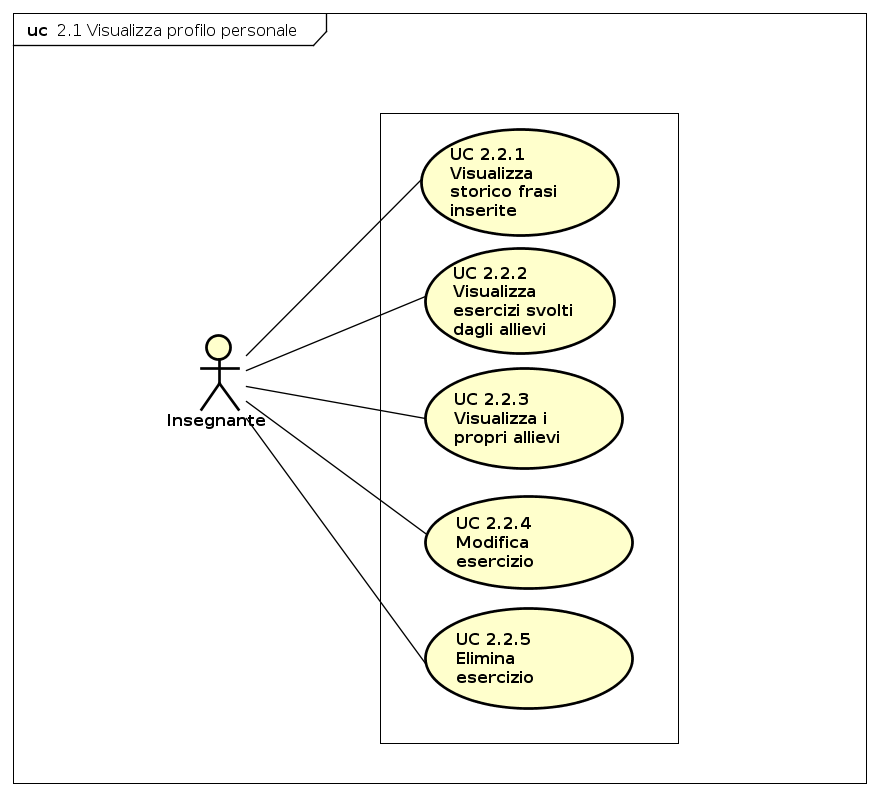
\includegraphics[width=17cm]{img/UC21.png} 
\caption{Caso d'uso UC2.1}
\end{figure}

\begin{itemize}
	\item[•] \textbf{Attori}: Utente non registrato;
	\item[•] \textbf{Descrizione}:  L’utente non registrato compila il form di registrazione relativo all’insegnante completando la registrazione;
	\item[•] \textbf{Precondizione}: L’utente non è registrato;
	\item[•] \textbf{Postcondizione}: L’utente si è registrato come insegnante;
	\item[•] \textbf{Flusso degli eventi}:
		\begin{enumerate}
			\item UC2.1.1 Inserimento nome utente;
			\item UC2.1.2 Inserimento email;
			\item UC2.1.3 Inserimento password;
			\item UC2.1.4 Inserimento conferma password;
			\item UC2.1.5 Inserimento data di nascita;
			\item UC2.1.6 Inserimento scuola di appartenenza;
			\item UC2.1.7 Inserimento materia insegnata.
		\end{enumerate}
	\item[•] \textbf{Estensioni}:
		\begin{enumerate}
			\item UC2.1.8 Errore utente omonimo.
		\end{enumerate}
\end{itemize}

\subsubsection{UC2.1.1 Inserimento nome utente}
\begin{itemize}
	\item[•] \textbf{Attori}: Utente non registrato;
	\item[•] \textbf{Descrizione}: L'utente non registrato inserisce il proprio nome utente nelle apposite caselle di testo;
	\item[•] \textbf{Precondizione}: L’utente non è registrato;
	\item[•] \textbf{Postcondizione}: L'utente ha inserito il proprio nome utente;
	\item[•] \textbf{Estensioni}:
		\begin{enumerate}
			\item UC2.1.8 Errore presenza di un utente omonimo
		\end{enumerate}
\end{itemize}

\subsubsection{UC2.1.2 Inserimento email istituzionale}
\begin{itemize}
	\item[•] \textbf{Attori}: Utente non registrato;
	\item[•] \textbf{Descrizione}: L'utente non registrato inserisce la propria mail istituzionale nell'apposita casella di testo;
	\item[•] \textbf{Precondizione}: L’utente non è registrato;
	\item[•] \textbf{Postcondizione}: L'utente ha inserito la propria mail istituzionale;	
	\item[•] \textbf{Estensioni}:
		\begin{enumerate}			
			\item UC2.1.8 Errore presenza utente omonimo.
		\end{enumerate}
\end{itemize}

\subsubsection{UC2.1.3 Inserimento password}
\begin{itemize}
	\item[•] \textbf{Attori}: Utente non registrato;
	\item[•] \textbf{Descrizione}: L'utente non registrato inserisce la propria password nell'apposita casella di testo;
	\item[•] \textbf{Precondizione}: L’utente non è registrato;
	\item[•] \textbf{Postcondizione}: L'utente ha inserito la propria password nell'apposita casella;
\end{itemize}

\subsubsection{UC2.1.5 Inserimento data di nascita}
\begin{itemize}
	\item[•] \textbf{Attori}: Utente non registrato;
	\item[•] \textbf{Descrizione}: L'utente non registrato inserisce la propria data di nascita nell'apposita casella di testo;
	\item[•] \textbf{Precondizione}: L’utente non è registrato;
	\item[•] \textbf{Postcondizione}: L'utente ha inserito la propria data di nascita;
	\item[•] \textbf{Estensioni}:
		\begin{enumerate}
			\item UC2.1.9 Data di nascita errata
		\end{enumerate}
\end{itemize}

\subsubsection{UC2.1.6 Inserimento scuola di appartenenza}
\begin{itemize}
	\item[•] \textbf{Attori}: Utente non registrato;
	\item[•] \textbf{Descrizione}: L'utente non registrato inserisce la propria scuola di appartenenza nell'apposita casella di testo;
	\item[•] \textbf{Precondizione}: L’utente non è registrato;
	\item[•] \textbf{Postcondizione}: L'utente ha inserito la scuola di appartenza;
\end{itemize}

\subsubsection{UC2.1.7 Inserimento materia insegnata}
\begin{itemize}
	\item[•] \textbf{Attori}: Insegnante;
	\item[•] \textbf{Descrizione}: L'utente non registrato inserisce la materia insegnata nell'apposita casella di testo;
	\item[•] \textbf{Precondizione}: L’utente non è registrato;
	\item[•] \textbf{Postcondizione}: L'utente ha inserito la materia insegnata;
\end{itemize}

\subsubsection{UC2.1.8 Errore presenza utente omonimo}
\begin{itemize}
	\item[•] \textbf{Attori}: Utente non registrato;
	\item[•] \textbf{Descrizione}:  L'utente non registrato sta provando a registrarsi come insegnante con un nome utente già presente all'interno del sistema;
	\item[•] \textbf{Precondizione}: L’utente non è registrato;
	\item[•] \textbf{Postcondizione}: Viene visualizzato un messaggio di errore;
\end{itemize}

\subsubsection{UC2.1.9 Data di nascita non valida}
\begin{itemize}
	\item[•] \textbf{Attori}: Utente non registrato;
	\item[•] \textbf{Descrizione}: L'utente non registrato sta provando a registrarsi come insegnante con una data di nascita errato o non valida;
	\item[•] \textbf{Precondizione}: L’utente non è registrato;
	\item[•] \textbf{Postcondizione}: Viene visualizzato un messaggio di errore;
\end{itemize}


\subsection{UC2.2 Visualizza profilo personale}

\begin{figure}[H]
\centering
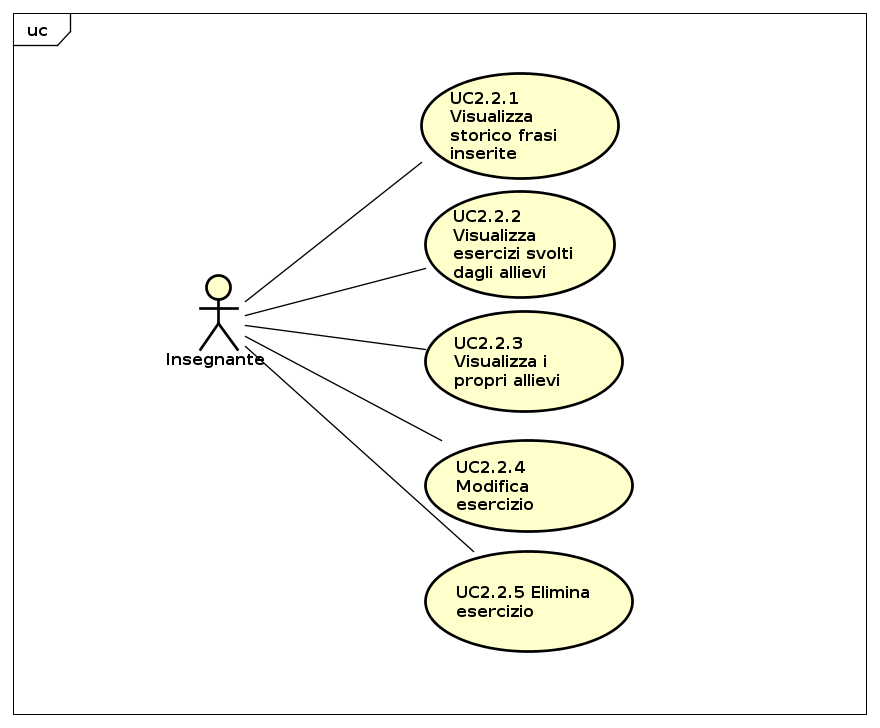
\includegraphics[width=14cm]{img/UC22.png} 
\caption{Caso d'uso UC2.2}
\end{figure}

\begin{itemize}
	\item[•] \textbf{Attori}: Insegnante;
	\item[•] \textbf{Descrizione}: L’insegnante visualizza il suo profilo personale;

	\item[•] \textbf{Precondizione}: Il sistema offre l’accesso a una dashboard con tutti i dati ;

	\item[•] \textbf{Postcondizione}:  Il profilo personale dell’insegnante è aperto;
	\item[•] \textbf{Flusso degli eventi}:
		\begin{enumerate}
			\item UC2.2.1 Visualizza storico frasi inserite;
			\item UC2.2.2 Visualizza esercizi svolti dagli allievi;
			\item UC2.2.3 Visualizza i propri allievi;
			\item UC2.2.4 Modifica esercizio;
			\item UC2.2.5 Elimina esercizio.
		\end{enumerate}
\end{itemize}

\subsubsection{UC2.2.1  Visualizza storico frasi inserite}

\begin{figure}[H]
\centering
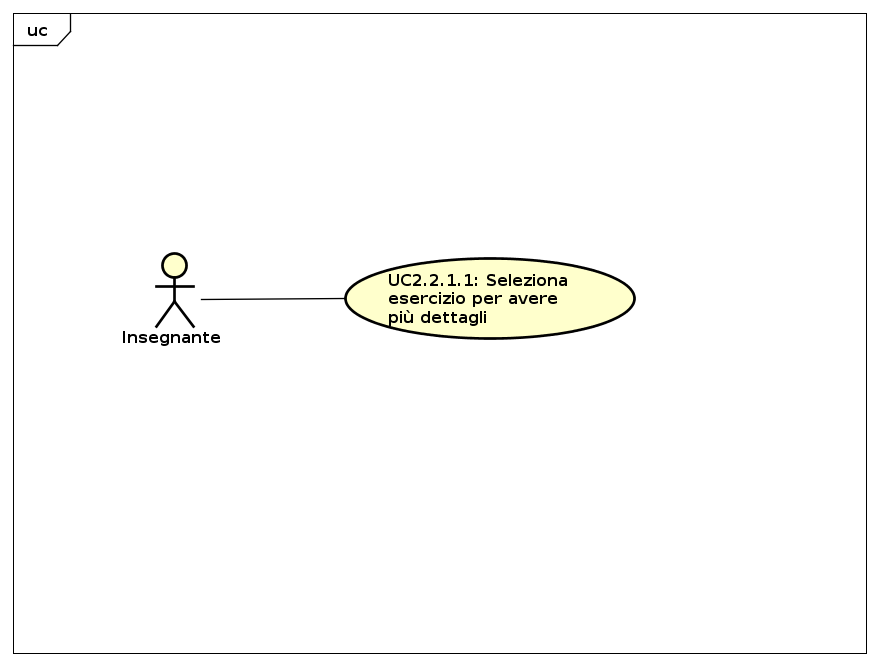
\includegraphics[width=10cm]{img/UC221.png} 
\caption{Caso d'uso UC2.2.1}
\end{figure}

\begin{itemize}
	\item[•] \textbf{Attori}:  Insegnante	\item[•] \textbf{Descrizione}: L’insegnante visualizza nel suo profilo personale lo storico delle frasi inserite; 
	\item[•] \textbf{Precondizione}: Il sistema offre la possibilità di visualizzare lo storico delle frasi inserite dall’insegnante;
	\item[•] \textbf{Postcondizione}:  L’insegnante può navigare all’interno della lista di frasi che ha inserito.
	\item[•] \textbf{Flusso degli eventi}:
		\begin{enumerate}
			\item UC2.2.1.1  Seleziona esercizio per avere più dettagli.
		\end{enumerate}
\end{itemize}

\subsubsection{UC2.2.1.1 Seleziona esercizio per avere più dettagli}
\begin{itemize}
	\item[•] \textbf{Attori}: Insegnante;
	\item[•] \textbf{Descrizione}:  L’insegnante seleziona dalla lista degli esercizi assegnati un esercizio e ne visualizza i dettagli;
	\item[•] \textbf{Precondizione}: Il sistema offre la possibilità di visualizzare i dettagli relativi ad un esercizio assegnato;
	\item[•] \textbf{Postcondizione}: L’insegnante legge le specifiche dell’esercizio selezionato.
\end{itemize}

\subsubsection{UC2.2.2  Visualizza esercizi svolti dagli allievi}
\begin{figure}[H]
\centering
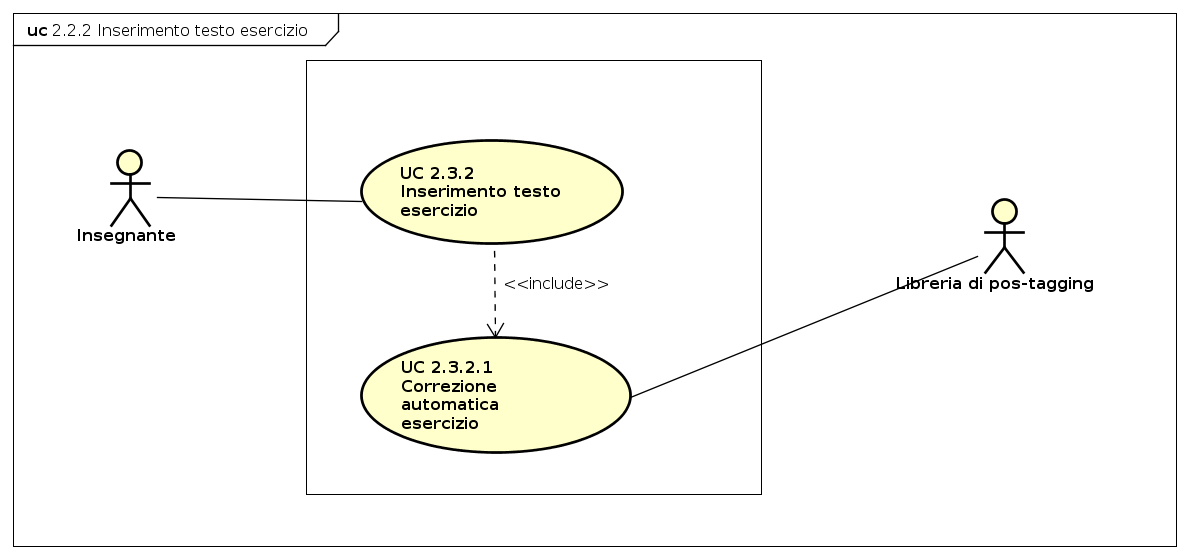
\includegraphics[width=10cm]{img/UC222.png} 
\caption{Caso d'uso UC2.2.2}
\end{figure}
\begin{itemize}
	\item[•] \textbf{Attori}: Insegnante;
	\item[•] \textbf{Descrizione}:  L’insegnante è nella sezione profilo personale ed entra
		nel registro che conserva gli esercizi svolti dagli allievi;
	\item[•] \textbf{Precondizione}:  L’insegnante ha degli allievi e ha assegnato a loro degli esercizi che sono stati svolti e consegnati;

	\item[•] \textbf{Postcondizione}: L’insegnante può navigare all’interno degli esercizi svolti 
                       svolti dagli allievi; 

	\item[•] \textbf{Flusso degli eventi}:
		\begin{enumerate}
			\item UC2.2.1.1  Seleziona esercizio specifico per avere più dettagli.	
		\end{enumerate}
\end{itemize}

\subsubsection{UC2.2.3 Visualizza i propri allievi}

\begin{figure}[H]
\centering
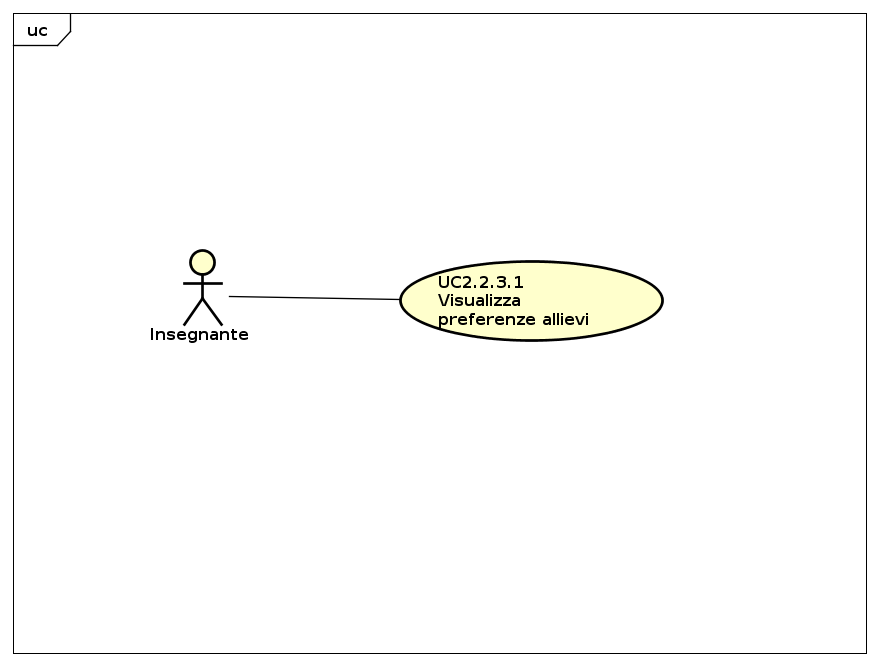
\includegraphics[width=10cm]{img/UC223.png} 
\caption{Caso d'uso UC2.2.3}
\end{figure}

\begin{itemize}
	\item[•] \textbf{Attori}: Insegnante;
	\item[•] \textbf{Descrizione}: L’insegnante visualizza la lista dei suoi allievi;
	\item[•] \textbf{Precondizione}: Il sistema offre all’insegnante di visualizzare la lista dei propri allievi;
	\item[•] \textbf{Postcondizione}: L’insegnante visualizza la lista dei propri allievi;
	\item[•] \textbf{Flusso degli eventi}:
		\begin{enumerate}
			\item UC2.2.3.1 Visualizza preferenze allievi.
		\end{enumerate}
\end{itemize}

\subsubsection{UC2.2.3.1 Visualizza preferenze allievi}
\begin{itemize}
	\item[•] \textbf{Attori}: Insegnante;
	\item[•] \textbf{Descrizione}: L’insegnante visualizza nel suo profilo personale le preferenze da parte degli allievi;
	\item[•] \textbf{Precondizione}: Il sistema offre la possibilità di poter segnare un insegnante come preferito;
	\item[•] \textbf{Postcondizione}: L’insegnante può vedere le preferenze degli allievi.
\end{itemize}


\subsubsection{UC2.2.4 Modifica esercizio}

\begin{figure}[H]
\centering
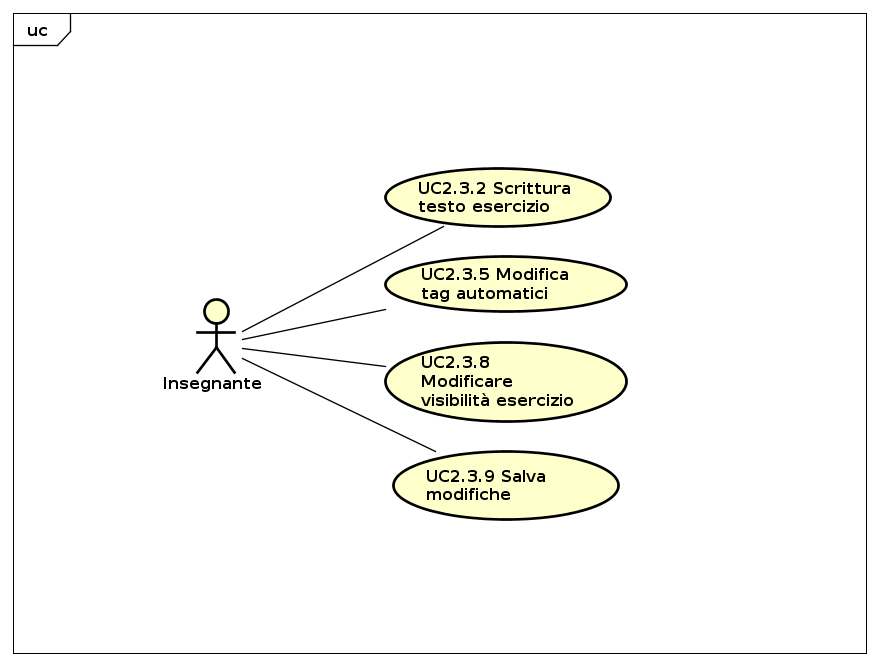
\includegraphics[width=10cm]{img/UC224.png} 
\caption{Caso d'uso UC2.2.4}
\end{figure}

\begin{itemize}
	\item[•] \textbf{Attori}: Insegnante;
	\item[•] \textbf{Descrizione}: L’insegnante può modificare un esercizio precedentemente inserito;
	\item[•] \textbf{Precondizione}: Il sistema offre la possibilità di modificare il testo, la
				lingua la visibilità i tag e le soluzioni alternative 
				dell’esercizio;
	\item[•] \textbf{Postcondizione}: L’esercizio è stato modificato;
	\item[•] \textbf{Flusso degli eventi}:
		\begin{enumerate}
			\item UC2.3.2 Scrittura testo esercizio;
			\item UC2.3.5 Modifica tag automatici;
			\item UC2.3.8 Modificare visibilità esercizio.
		\end{enumerate}
		    
\end{itemize}   	
	
\subsubsection{UC2.2.5 Elimina esercizio}
\begin{itemize}
	\item[•] \textbf{Attori}: Insegnante;
	\item[•] \textbf{Descrizione}: L’insegnante elimina un esercizio che è stato assegnato;
	\item[•] \textbf{Precondizione}: Il sistema offre la possibilità di eliminare un esercizio che è stato assegnato;
	\item[•] \textbf{Postcondizione}: L’esercizio assegnato è stato cancellato.
\end{itemize}

%%%%%%%%%%%%%%%%%%%%%%%%%%%%%%%%%%%%%%%%%%%%%%%%%%%%%%%%%%%%%%%%%%%%%%%%%%%%%%%%%%%%%%%%%%%%%%%%%%%%%%%%%%%%%%%%%%

  %%%%%%%%%%%%		PARTE STEFANO		%%%%%%%%%%%%%

%%%%%%%%%%%%%%%%%%%%%%%%%%%%%%%%%%%%%%%%%%%%%%%%%%%%%%%%%%%%%%%%%%%%%%%%%%%%%%%%%%%%%%%%%%%%%%%%%%%%%%%%%%%%%%%%%%

\subsection{UC2.3 Inserimento di un nuovo esercizio}
\begin{itemize}
	\item[•] \textbf{Attori}: Insegnante;
	\item[•] \textbf{Descrizione}: Insegnante attraverso una form aggiunge il testo di un nuovo esercizio;
	\item[•] \textbf{Precondizione}: Il sistema offre la possibilità di aggiungere un esercizio nel sistema;
	\item[•] \textbf{Postcondizione}: Un nuovo esercizio è stato aggiunto;
	\item[•] \textbf{Flusso degli eventi}:;
	\begin{enumerate}
		\item UC2.3.1 Predisporre lingua esercizio
		\item UC2.3.2 Scrittura testo esercizio
		\item UC2.3.3 Correzione automatica esercizio
		\item UC2.3.4 Modifica tag automatici
		\item UC2.3.5 Inserire più soluzioni
		\item UC2.3.6 Modificare visibilità esercizio
		\item UC2.3.7 Salva modifiche
		\item UC2.3.1.1	Conferma aggiunta esercizio
	\end{enumerate}
	\item[•] \textbf{Estensioni}:	
	\begin{enumerate}
		\item UC2.3.8 Visualizzazione errori
	\end{enumerate}
\end{itemize}

\subsubsection{UC2.3.1 Predisporre lingua esercizio}
\begin{itemize}
	\item[•] \textbf{Attori}: Insegnante;
	\item[•] \textbf{Descrizione}: Insegnante sceglie la lingua dell’esercizio che vuole scrivere;
	\item[•] \textbf{Precondizione}: Il sistema offre la possibilità di scegliere tra più lingue il testo 
			dell’esercizio;
	\item[•] \textbf{Postcondizione}: La lingua è stata scelta;
\end{itemize}

\subsubsection{UC2.3.2 Scrittura testo esercizio}
\begin{itemize}
	\item[•] \textbf{Attori}: Insegnante;
	\item[•] \textbf{Descrizione}: Insegnante scrive il testo dell’esercizio;
	\item[•] \textbf{Precondizione}: Il sistema offre la possibilità di scrivere un testo;
	\item[•] \textbf{Postcondizione}: Il testo è stato scritto;
	\item[•] \textbf{Flusso degli eventi}:
	\begin{enumerate}
		\item UC2.3.1.1	Cancellazione ultimo carattere
		\item UC2.3.1.2	Testo esercizio completato
	\end{enumerate}
	\item[•] \textbf{Estensioni}:	
	\begin{enumerate}
		\item UC2.3.3 Interruzione scrittura testo esercizio.
	\end{enumerate}
\end{itemize}


\subsubsection{UC2.3.3	Correzione automatica esercizio}
\begin{itemize}
	\item[•] \textbf{Attori}: Insegnante e libreria di pos-tagging;
	\item[•] \textbf{Descrizione}: L’Insegnante genera automaticamente i tag dal testo dell’ esercizio;
	\item[•] \textbf{Precondizione}: Il sistema offre la possibilità di scrivere un testo e generare dei tag grammaticali per ogni parola del testo;
	\item[•] \textbf{Postcondizione}: I tag relativi al testo scritto sono stati generati;
\end{itemize}

\subsubsection{UC2.3.4	Modifica tag automatici}
\begin{itemize}
	\item[•] \textbf{Attori}: Insegnante e libreria di pos-tagging;
	\item[•] \textbf{Descrizione}: L’Insegnante modifica/corregge i tag generati automaticamente;
	\item[•] \textbf{Precondizione}: Il sistema offre la possibilità di modificare i tag generati con la correzione automatica;
	\item[•] \textbf{Postcondizione}: I tag relativi al testo scritto sono stati modificati o corretti;
	\item[•] \textbf{Estensioni}:
	\begin{enumerate}
		\item UC002.6 Interruzione modifica/correzione dei tag
	
	\end{enumerate}
\end{itemize}

\subsubsection{UC2.3.5	Inserire più soluzion}
\begin{itemize}
	\item[•] \textbf{Attori}: Insegnante e libreria di pos-tagging;
	\item[•] \textbf{Descrizione}: Insegnante inserisce tag alternativi all’esercizio consultando la libreria di pos-tagging;
	\item[•] \textbf{Precondizione}: Il sistema offre la possibilità di inserire più tag per parola ad 
			esercizio;
	\item[•] \textbf{Postcondizione}: Una soluzione alternativa è stata aggiunta;
\end{itemize}

\subsubsection{UC2.3.6	Modificare visibilità esercizio}
\begin{itemize}
	\item[•] \textbf{Attori}: Insegnante;
	\item[•] \textbf{Descrizione}: Insegnante decide chi può visualizzare e svolgere esercizio;
	\item[•] \textbf{Precondizione}: Il sistema offre la possibilità di monitorare visibilità esercizio;
	\item[•] \textbf{Postcondizione}: L’esercizio è stato reso visibile o meno ad un gruppo di utenti;	
\end{itemize}

\subsubsection{UC2.3.7	Salva modifiche}
\begin{itemize}
	\item[•] \textbf{Attori}: Insegnante;
	\item[•] \textbf{Descrizione}: Insegnante salva esercizio e possibili modifiche;
	\item[•] \textbf{Precondizione}: Il sistema offre la possibilità di salvare gli esercizi creati;
	\item[•] \textbf{Postcondizione}: Un esercizio è stato salvato;
\end{itemize}

\subsubsection{UC2.3.8 Visualizzazione errori}
\begin{itemize}
	\item[•] \textbf{Attori}: Insegnante;
	\item[•] \textbf{Descrizione}: Insegnante visualizza gli errori relativi alla sintassi e la forma dell’esercizio che sta creando;
	\item[•] \textbf{Precondizione}: Il sistema offre la possibilità di visualizzare gli errori effettuati nella scrittura del testo ;
	\item[•] \textbf{Postcondizione}: L’esercizio è stato visionato dal sistema, e gli errori sono stati visualizzati;
\end{itemize}

\subsubsection{UC2.3.1.1 Conferma aggiunta esercizio}
\begin{itemize}
	\item[•] \textbf{Attori}: Insegnante;
	\item[•] \textbf{Descrizione}: Insegnante aggiunge un esercizio al sistema;
	\item[•] \textbf{Precondizione}: Il sistema offre la possibilità di aggiungere un esercizio;
	\item[•] \textbf{Postcondizione}: L’esercizio è stato aggiunto correttamente al sistema;
\end{itemize}

%\subsection{•}
%\begin{itemize}
%	\item[•] \textbf{Attori}:;
%	\item[•] \textbf{Descrizione}:;
%	\item[•] \textbf{Precondizione}:;
%	\item[•] \textbf{Postcondizione}:;
%	\item[•] \textbf{Flusso degli eventi}:;
%	\begin{enumerate}
%		\item
%		\item
%	\end{enumerate}
%	\item[•] \textbf{Estensioni}:;	
%	\begin{enumerate}
%		\item
%		\item
%	\end{enumerate}
%\end{itemize}





